\documentclass[]{templateWYC}
\usepackage{multicol}

\title{报告标题}
\author{作者}
\affil{下北泽大学$\quad$2020114514}
\date{\today}

\newredbox{问题}{prob}
\newblackbox{注意}{notice}

\begin{document}
	\maketitle

	\begin{abstract}
		一段摘要正文。

		另一段摘要正文。
	\end{abstract}

	\section{某一节}\label{sec:1}
		实验仪器包括 WGD30 型光栅单色仪,汞灯,溴钨灯,三路输出电源,光电探测器(量程2\si{\volt}),
		样品(安装有0.5\si{\milli\metre}和1\si{\milli\metre}两种厚度的钕玻璃吸收片),显微镜(放大倍数20),
		聚光镜(焦距 $f = 60\si{\milli\metre}$,通光孔径$d = 30\si{\milli\metre}$)。

	\section{又一节}
	\subsection{一个小节}
		\begin{wrapfigure}{r}{0.32\textwidth}
			\centering
			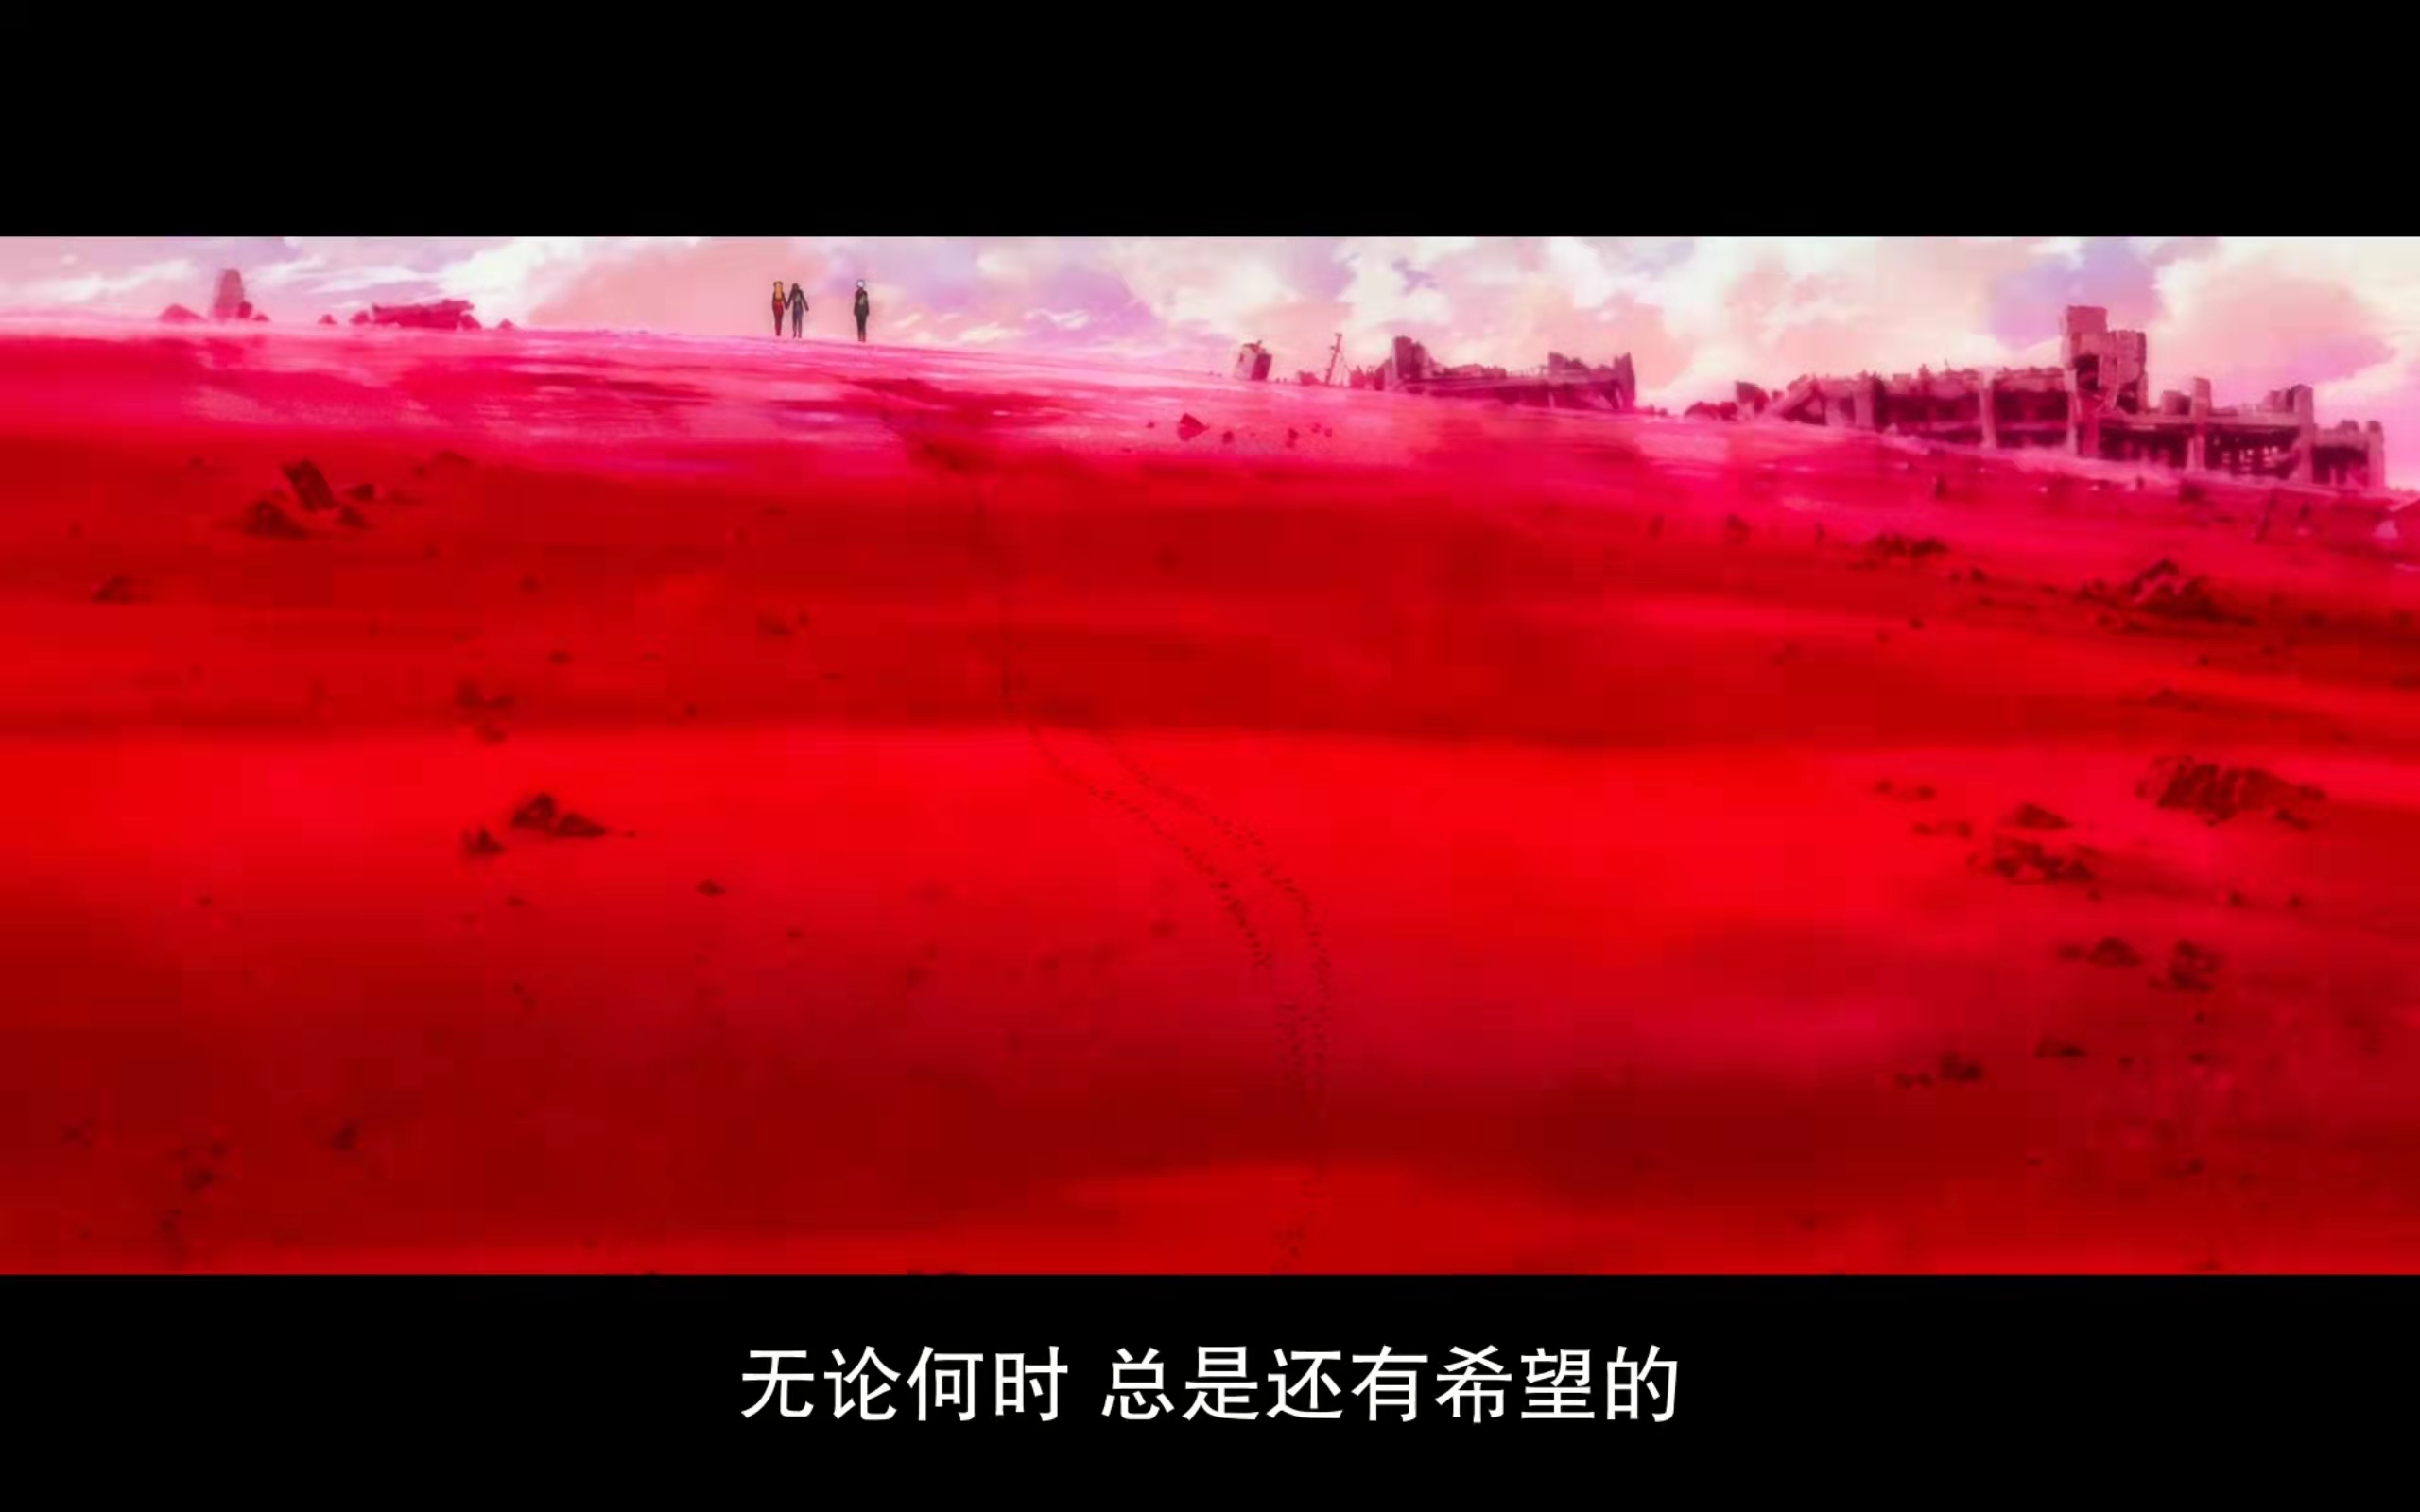
\includegraphics[width=0.32\textwidth]{sample.jpg}
			\caption{示例图片}\label{fig:1}
		\end{wrapfigure}

		此处为文字内容文字内容文字内容文字内容文字内容文字内容文字内容文字内容
		文字内容文字内容文字内容文字内容文字内容文字内容文字内容文字内容
		文字内容文字内容文字内容文字内容文字内容文字内容文字内容文字内容
		文字内容文字内容文字内容文字内容文字内容文字内容文字内容文字内容
		文字内容文字内容文字内容文字内容文字内容文字内容文字内容文字内容
		文字内容文字内容文字内容文字内容文字内容。

		此处为公式示例:$\dfrac{\partial \bm{n}}{\partial \xi^\alpha}=-b_{\alpha\beta}\bm{\rho}^\beta$,
		这是因为
		\begin{align*}
			&\frac{\partial \bm{n}}{\partial \xi^\alpha}\cdot\bm{\rho}_\beta\\
			=&\frac{\partial}{\partial \xi^\alpha}(\bm{n}\cdot\bm{\rho}_\beta) - \bm{n}\cdot\frac{\partial \bm{\rho}_\beta}{\partial \xi^\alpha}\\
			=&-b_{\alpha\beta}
		\end{align*}
		
		\subsection{一个新的小节}
		在\cref{sec:1}中插入了\cref{fig:1}。

	\section{再一节}

		\begin{prob}[一种box示例]
			环境标题可在模板中修改。
		\end{prob}
		\begin{prob*}
            不带编号的相应box。
        \end{prob*}

		\begin{notice}[另一种box示例]
			此处为文字内容。
		\end{notice}

	\section{最后一节}
	pgf绘图示例如\cref{fig:2}所示。不建议直接使用pgf。
	\begin{figure}[h]
		\centering
        \begin{tikzpicture}
            \begin{axis}[
                xlabel={波长$\lambda$ [\si{\nano\metre}]},
                ylabel={吸收系数$\alpha$ [\si{\milli\metre^{-1}}]},
                xmin=500, xmax=620,
                ymin=0, ymax=5,
                major x tick style = {opacity=1},
                minor x tick num = 9,
                %minor y tick num = 9,
                legend pos=north east,
                grid=both,
            ]
                
            \addplot[color=blue,mark=circle]
                coordinates {
                    (510.6,0.5022)
                    (512.6,0.6444)
                    (514.6,0.6710)
                    (516.6,0.5907)
                    (518.6,0.5236)
                    (520.6,0.5426)
                    (522.6,0.7040)
                    (524.6,0.9329)
                    (526.6,1.0818)
                    (528.6,1.1200)
                    (530.6,1.0395)
                    (532.6,0.8934)
                    (534.6,0.6559)
                    (536.6,0.4289)
                    (538.6,0.2943)
                    (540.6,0.1606)
                    (542.6,0.1239)
                    (544.6,0.0753)
                    (546.6,0.0618)
                    (548.6,0.0458)
                    (550.6,0.0412)
                    (552.6,0.0370)
                    (554.6,0.0478)
                    (556.6,0.0502)
                    (558.6,0.0606)
                    (560.6,0.0740)
                    (562.6,0.1004)
                    (564.6,0.1832)
                    (566.6,0.3750)
                    (568.6,0.8533)
                    (569.5,1.2785)
                    (570.0,1.5961)
                    (570.5,1.8648)
                    (571.0,2.1745)
                    (571.5,2.4671)
                    (572.0,2.7964)
                    (572.5,3.0066)
                    (573.0,3.1163)
                    (573.5,3.2093)
                    (574.0,3.2447)
                    (574.5,3.2543)
                    (575.0,3.2569)
                    (575.5,3.2690)
                    (576.0,3.2466)
                    (576.5,3.1888)
                    (577.0,3.1716)
                    (577.5,3.1244)
                    (578.6,3.0921)
                    (580.6,3.1416)
                    (581.3,3.2274)
                    (581.8,3.3817)
                    (582.3,3.5561)
                    (582.8,3.8029)
                    (583.3,4.0453)
                    (583.8,4.2105)
                    (584.3,4.4492)
                    (584.8,4.5696)
                    (585.3,4.5374)
                    (585.8,4.5535)
                    (586.3,4.4791)
                    (586.8,4.3831)
                    (587.3,4.2658)
                    (587.8,4.0298)
                    (588.3,3.9308)
                    (588.8,3.6583)
                    (589.3,3.4760)
                    (590.6,3.1446)
                    (592.6,2.6130)
                    (594.6,2.0122)
                    (596.6,1.4953)
                    (598.6,1.1410)
                    (600.6,0.8892)
                    (602.6,0.6560)
                    (604.6,0.4753)
                    (606.6,0.3658)
                    (608.6,0.2784)
                    (610.6,0.2063)
                };
            \end{axis}
        \end{tikzpicture}
		\caption{绘图示例}\label{fig:2}
	\end{figure}


\end{document}